\newpage
\section{Use case diagram}
\begin{figure}[hbt!]
	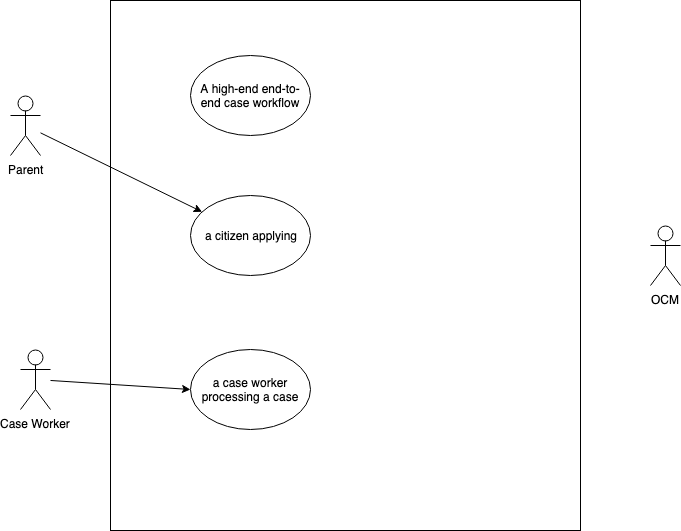
\includegraphics[width=\textwidth]{img/use-cases}
	\caption{Use case diagram}
\end{figure}

\newpage
\section{Detailed Use cases}

\subsection{UC01: A high-end end-to-end case workflow}

\begin{table}[htb!]
\begin{tabularx}{\textwidth}{l|X}
	\textbf{Use Case name} & A high-end end-to-end case workflow \\
	\hline
	\textbf{Participating actor} & Caseworker, User\\
	\hline
	\textbf{Flow of events} &
	\begin{compactenum}
			\item User creates application for loss of earnings,provides all needed information.
			\item Caseworker receives application, processes it and approves it.
			\item OCM sends email about the the approval of the application
			\item Calculation of compensation will be made by OCM
			\item OCM sets application on done
	\end{compactenum}\\
	\hline
	\textbf{Extensions} & 
	    \begin{compactenum}
	        \setcounter{enumi}{1}
	        \item \begin{compactenum}
	            \item Caseworker rejects application
	            \item OCM sends mail of rejection
	        \end{compactenum}
	    \end{compactenum}\\
	\hline
	\textbf{Entry condition} &
	Caseworker is logged in
	\\
	\hline
	\textbf{Exit condition} & 
	\begin{compactenum}
	    \item Caseworker is logged out
	\end{compactenum}
	\\
	\hline
	\textbf{Quality requirements} & See non-functional requirements in section \ref{sec:nfr}\\
\end{tabularx}
\end{table}

\subsection{UC02: A citizen applying}

\begin{table}[htb!]
\begin{tabularx}{\textwidth}{l|X}
	\textbf{Use Case name} & A citizen applying \\
	\hline
	\textbf{Participating actor} & User\\
	\hline
	\textbf{Flow of events} & 
	    \begin{compactenum}
	        \item User visits the portal
	        \item User initiates the process for applying loss of earnings
	        \item User fills out all the necessary information needed in the form
	        \item User uploads all required documentation
	        \item User uploads a doctor confirmation
	    \end{compactenum}\\
	\hline
	\textbf{Entry condition} & User is logged in\\
	\hline
	\textbf{Exit condition} & User saves the application and logs out\\
	\hline
	\textbf{Quality requirements} & See non-functional requirements in section \ref{sec:nfr}\\
\end{tabularx}
\end{table}

\subsection{UC03: A case worker processing a case}
\begin{table}[htb!]
\begin{tabularx}{\textwidth}{l|X}
	\textbf{Use Case name} & A case worker processing a case \\
	\hline
	\textbf{Participating actor} & Caseworker\\
	\hline
	\textbf{Flow of events} & 
	    \begin{compactenum}
	        \item Caseworker opens a newly opened application
	        \item Caseworker checks the documentation to be legitimate (including the provided doctor confirmation)
	        \item Caseworker approves application
	        \item OCM calculates 
	    \end{compactenum}\\
	\hline
	\textbf{Entry condition} & Caseworker is logged in\\
	\hline
	\textbf{Exit condition} & \\
	\hline
	\textbf{Quality requirements} & See non-functional requirements in section \ref{sec:nfr}\\
\end{tabularx}
\end{table}